\section{Problem}


Now that our snake robot is capable of moving through the environment with the adaptive concertina gait behavior, we need some way of estimating how far it is moving and in which direction.

As we established earlier, we have no external sensors because we assume their failure from environmental conditions.  We cannot rely on GPS since it is not effective underground or in pipes.  We do not have wheeled shaft encoders since we have no wheels and do not expect to always travel through flat terrain.  Finally, although it may indeed help, we cannot expect to make use of an inertial navigation system since they are bulky and expensive.  Furthermore, we have not performed experiments to determine if they are capable of handling the high amount of rotation of each of the snake body segments during locomotion.

In absence of a global positioning or odometry, we need some form of alternative motion estimation. Knowing where the robot is located is the basic building block of creating a map.  We focus on the problem of finding the relative geometric transform between the two poses at the beginning and end of one step of the adaptive concertina gait. 

Our proprioceptive approach achieves motion estimation by anchoring multiple points of the body with the environment and kinematically tracking the change in distance between the immobilized parts as the snake contracts and extends.  This gives us a motion estimation method that only depends on the joint sensors.  We show the effectiveness in a series of experiments.
 

\section{Immobilizing the Anchors}

\label{sec:anchors}

%-Immobilize anchors to create global references
%-Conditions when immobility or anchor slip occurs
%-How to know when immobilized (heuristics)

A fundamental property of the adaptive concertina gait is that it creates anchors to the surrounding environment.  Our goal is to exploit this property to estimate our motion through the environment.  In order to do this, we need to ensure that our anchors remain an accurate frame of reference to the global environment.

The primary goal of our previous work on maintaining smooth and stable motion of the snake in Chapter 2 was to prevent any sort of anchor slip that may harm our reference frame to the global environment.  It is critical that our anchors remain firmly immobilized with respect to the environment to ensure accurate measurement of motion.

Though we are not able to localize the exact contact point of the anchor with the environment, we can assume that the segments comprising the anchoring curve are themselves immobilized and mechanically isolated by virtue of their static contacts with the environment.  We use these isolated bodies as immobilized references to the global environment.

Whether or not we consider the use of a body segment as a reference is determined by our work in Section 2.8.  That is, if the joints in the local neighborhood of a segment are locally stable and the behavior's control bit for the attached joint is 0, we assume this segment is immobilized.  We can use immobilized segments as reference points to the global frame.

We call the monitoring of local joint variances as local stability and the output of the control masks as prescriptive stability.  Though a body segment may be locally stable, it does not mean it is immobile.  If we also include prescriptive stability, the behavior's prediction of what joints should be moving and what should not, then we greatly decrease the chances that we will use a slipping anchor as a reference.

If any point the anchor should slip while, our assumption that a body segment is immobilized is violated and could lead to accumulated errors in our motion technique.  Therefore, it is critical that we analyze and mitigate all the possible failure modes for anchoring.

We are generally able to classify the types of anchoring and reference errors we encounter during both static and locomotive anchoring.  For each, we are forced to either avoid the condition from occurring or detect and correct it. We list the failure modes and explain our mitigation strategy for each.

The \emph{floating reference} occurs when a locally stable segment is made a reference, but it is not part of an anchor. This was particularly troublesome in our early implementations, but we are able to largely avoid this failure mode by having the behaviors explicitly classifying which joints are part of an anchor. The other possibility for a floating anchor would be if an anchoring behavior erroneously reports success in establishing an anchor in free space. This was largely avoided by adding the more careful anchoring process in Section 2.2 that detects impacts to the walls and follows up by doing a jerk test to test whether the anchor is secure.

A \emph{weak contact} occurs when the anchor the reference segment is on has an insecure anchor. This usually happens if an anchor is placed within a pipe junction or if one of the anchors of the Back-Anchor is insecure.  The Back-Anchor case is more likely since they are not jerk-tested.  Weak contacts usually do not display local instability since the physical contact stabilizes the local joints but does not immobilize them.  If it is available, we can use negative prescriptive stability from the behavior to minimize this failure but often occurs in prescriptively stable areas.  There is nothing we can do to prevent this error from being added to the pose estimation besides detecting it.  Luckily, a weak contact does not move much.  Its error is bounded.

\emph{Buckling} occurs when the anchored joints are frozen in a non-optimal position and external stresses put excessive torque on one or more joints that forces the anchor into a reconfigured position. This is similar to mechanical buckling of structural members under compression.  In this case, it is for an articulated system attempting to hold a rigid pose. Buckling is easily detectable by tripping our local stability conditions and will quickly remove the references and reuse them once the joints have settled down. We have also reduced this occurrence by having our anchoring behaviors search for non-deforming anchors as a natural by-product of algorithm 2.

\emph{Impulses} occur when the snake robot experiences a sudden collision or a buckling has occurred somewhere else in the robot. Usually this is not a fatal error and the robot will quickly return to its stable pose. However it can trip up the variance calculations and deactivate all the references we have leaving us with none. Recovery is achieved by resurrecting the last best reference, and assuming it is in the same pose.  We show how to do this in the next section.

\emph{Funnel anchoring} occurs when a secure anchor is established between a pair of walls that are monotonically increasing in width. If the anchor receives a force that pushes it towards the direction of increasing width, its anchor can become permanently loose. This is especially problematic in cases of irregular environments where there are many possibilities for this to occur in local conditions. We currently do not have a solution for this yet.

Finally there is a class of \emph{whole body slip} that is completely undetectable with only joint positions. That is, the whole body could be slipping through an environment such as a straight and featureless pipe without causing any joint variance at all. This would only occur if the ground was exceptionally slippery and able to use the robot's momentum to move it large distances or if the robot was on a slope and gravity was exerting a global force. We avoid this error by limiting the environments we explore. Other environments may require extra sensor instrumentation such as accelerometers to detect this failure mode.

Rotational error is the dominant form of error we encounter because, unlike a traditional robot with a stable frame of reference on its chassis, every reference point in the snake robot's body is constantly in rotational motion. Any form of disturbance of a reference node will manifest itself with a rotational error that will propagate through kinematic computations of new reference nodes. Translational error occurs primarily by anchor slip.  Rotational error is easier to correct in our later localization process in Chapter 5.

\section{Tracking Motion}

%-What a reference is
%-each active reference can be used to compute the pose of the snake at that given time
%-active references may disagree with each other
%-take current oldest active reference to compute current pose
%-How to create new references (kinematic computation)
%-When to deactivate references (violation of local/pre stability)
%-Loss of all references recovery

In order to track motion through the environment, we need to establish our mathematical framework for defining the relative position of things between the robot and the environment.  We then define the concept of a \emph{reference pose} to track the position of the environment while the snake is in motion.

\subsection{Pose and Coordinate Frames}

\begin{figure}
\begin{center}
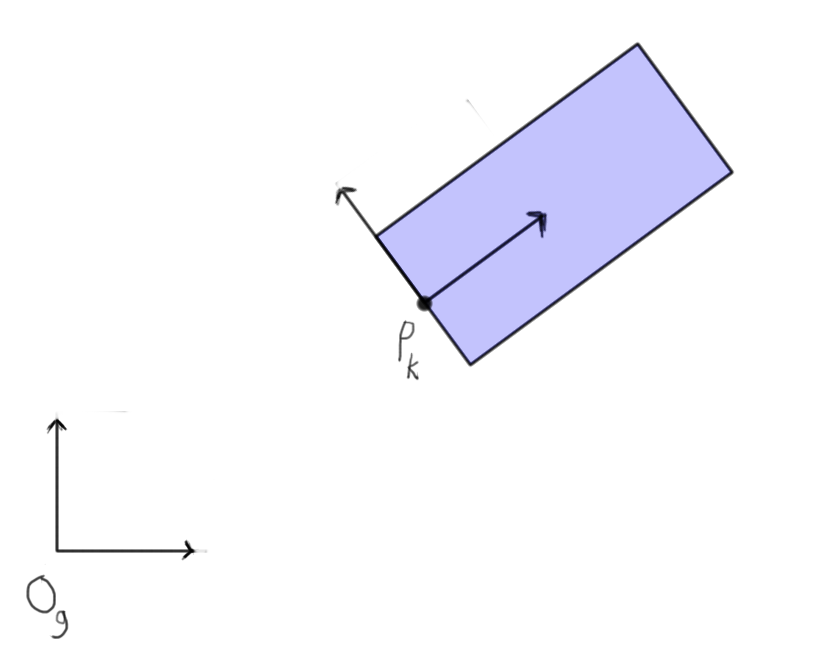
\includegraphics[scale=0.5]{3_pose_frame1.png}
\end{center}
\caption{Pose of rigid body with respect to global frame.}
\label{fig:pose_frame1}
\end{figure}

A pose $P$ defines the position and orientation of a rigid body in a 2D plane.  Each pose is defined with respect to a coordinate frame $O$ using 3 values: $(x,y,\theta)$.  A coordinate frame is either affixed in the global environment or affixed to a rigid body on the snake.  An example of the global frame $O_g$ and a pose $P_k$ are shown in Figure \ref{fig:pose_frame1}.

By convention, we will specify in the superscript which coordinate frame a pose $k$ is defined with respect to.  For the global frame, the pose is written as $P_k^g$.  If the pose is with respect to some other coordinate frame $O_a$, the pose is written as $P_k^a$.  If the superscript is omitted, we assume the global frame.

\begin{figure}
\begin{center}
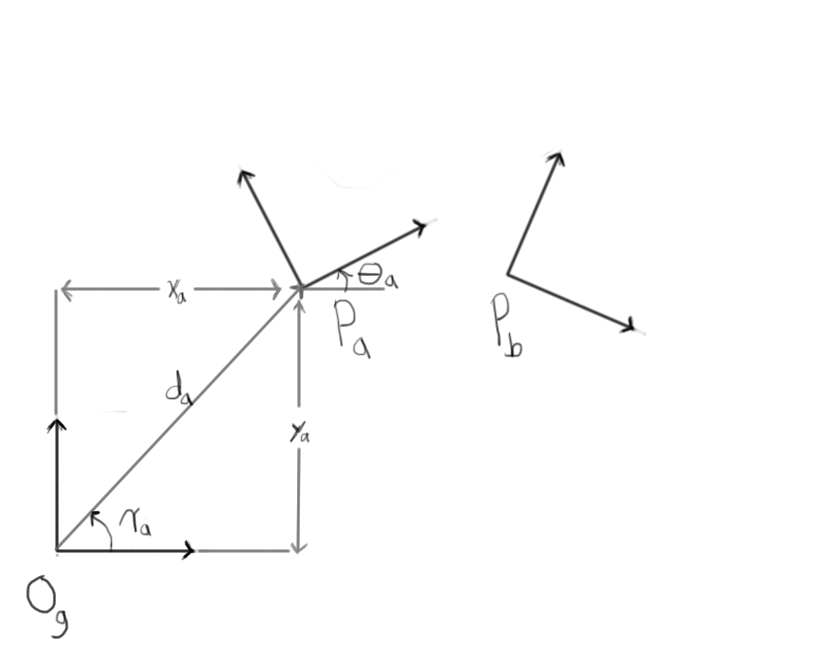
\includegraphics[scale=0.5]{3_pose_frame2.png}
\end{center}
\caption{Pose of A and B with respect to global frame.}
\label{fig:pose_frame2}
\end{figure}

In a robot system with multiple rigid bodies, we will have a coordinate frame for each body.  Often times, we wish to transform poses between coordinate frames.  To do this, we first need to define the relationship between coordinate frames, specified by the pose of their origins.  In the global frame $O_g$, the pose of the origin $O_g$ is $P_g = (0,0,0)$.  For two example coordinate frames attached to rigid bodies, we define the pose of origin $O_a$ to be $P_a = (x_a, y_a, \theta_a)$ and the pose of origin $O_b$ to be $P_b = (x_b, y_b, \theta_b)$ as shown in Figure \ref{fig:pose_frame2}.

Suppose we wanted to compute pose $b$ with respect to frame $O_a$.  That is, we wish to find $P_b^a$ and we are given $P_a^g$ and $P_b^g$.  First we focus on finding the Cartesian component of the pose, point $p_b^a = (x_b^a, y_b^a)$.  We compute the angle portion $\theta_b^a$ separately.  From Figure \ref{fig:pose_frame2}, we define the following:
\begin{equation}
\label{equ:coord1}
R_a =
\begin{bmatrix}
cos(\theta_a) & sin(\theta_a) \\
-sin(\theta_a) & cos(\theta_a)
\end{bmatrix}
\end{equation}

This is the rotation matrix for the difference in orientation between the global frame $O_g$ and local frame $O_a$.
\begin{equation}
\label{equ:coord2}
d_a = \sqrt{(x_a)^2 + (y_a)^2} 
\end{equation}

This is the Cartesian distance from the global frame's origin to the local frame's origin.
\begin{equation}
\cos(\gamma_a) = \frac{(x_a,y_a) \cdot (1,0)}{|(x_a, y_a)| |1|} = \frac{x_a}{d_a} 
\end{equation}
\begin{equation}
\label{equ:coord3}
\gamma_a = s \cdot \arccos \left( \frac{x_a}{d_a} \right) 
\quad
\left\{ 
  \begin{array}{l l}
    s = 1 & \quad \text{if $y_a \geq 0$}\\
    s = -1 & \quad \text{if $y_a < 0$}
  \end{array} \right.
\end{equation}

$\gamma_a$ is the angle of the vector from the global origin to the local frame origin.  The sign of $\gamma_a$ is determined to be negative if $y_a < 0$.  Otherwise, $\gamma_a$ is positive.  This value corresponds to the angle shown in Figure \ref{fig:pose_frame2}.
\begin{equation}
\label{equ:coord4}
G_a = 
\begin{bmatrix}
cos(\gamma_a) & sin(\gamma_a) \\
-sin(\gamma_a) & cos(\gamma_a)
\end{bmatrix}
\end{equation}

$G_a$ is the rotation matrix to rotate the local frame's origin onto the x-axis of the global frame.

To find $p_b^a$ in frame $O_a$ from $p_b^g$ in $O_g$, we compute:
\begin{equation}
\label{equ:g_to_c_cart}
p_b^a =
\begin{bmatrix}
x_b^a \\
y_b^a \\
\end{bmatrix}
 = R_a {G_a}^{\mathbf{T}} \left(G_a p_b^g 
-
\begin{bmatrix}
d_a \\
0
\end{bmatrix}
\right)
\end{equation}

To find the converse, $p_b^g$ from $p_b^a$, we do the following:
\begin{equation}
\label{equ:c_to_g_cart}
p_b^g =
\begin{bmatrix}
x_b^g \\
y_b^g \\
\end{bmatrix}
 = {G_a}^{\mathbf{T}} \left(
\begin{bmatrix}
d_a \\
0
\end{bmatrix}
+ G_a {R_a}^{\mathbf{T}} p_b^a \right)
\end{equation}

This approach performs a sequence of rotations to separate translation and rotation of the pose when converting between frames.  To compute the angle portion of the pose, we perform the rotation sequence by addition and subtraction of angles.  Following the sequence, we get the following: 
\begin{equation*}
\theta^a_b = \theta_b^g + \gamma_a - \gamma_a - \theta_a
\end{equation*}
This reduces to:
\begin{equation}
\label{equ:g_to_c_ori}
\theta^a_b = \theta_b^g - \theta_a
\end{equation}

The converse is achieved similarly using Equation \ref{equ:c_to_g_cart} and the following rotation sequence:
\begin{equation*}
\theta_b^g = \theta_b^a + \theta_a + \gamma_a - \gamma_a 
\end{equation*}
\begin{equation}
\label{equ:c_to_g_ori}
\theta_b^g = \theta_b^a + \theta_a
\end{equation}

The final result for the pose computation is to put the Cartesian and angular components together.
\begin{equation}
P_b^a =
\begin{bmatrix}
x_b^a \\
y_b^a \\
\theta_b^a 
\end{bmatrix}
\quad
\left\{ 
  \begin{array}{l l}
    x_b^a,y_b^a & \quad \text{from Equation \ref{equ:g_to_c_cart}}\\
    \theta_b^a & \quad \text{from Equation \ref{equ:g_to_c_ori}}
  \end{array} \right.
\end{equation}
And the converse is:
\begin{equation}
P_b^g =
\begin{bmatrix}
x_b^g \\
y_b^g \\
\theta_b^g 
\end{bmatrix}
\quad
\left\{ 
  \begin{array}{l l}
    x_b^g,y_b^g & \quad \text{from Equation \ref{equ:c_to_g_cart}}\\
    \theta_b^g & \quad \text{from Equation \ref{equ:c_to_g_ori}}
  \end{array} \right.
\end{equation}


Now that we have established the mathematical framework for relating the pose of the rigid bodies to the environment and each other, we describe our concept of reference poses to track motion in the environment.


\subsection{Reference Poses}

A reference pose is the position and orientation of a rigid body segment that has been immobilized with respect to the global frame.  A reference pose is valuable because it gives a fixed reference point to the global environment and allows us to track the motion of the rest of the robot.   Special care must be taken to ensure that when using a reference pose, the rigid body it's attached to is truly immobilized.

A reference pose is either active or inactive.  A reference is active once it is created as a result of its rigid body becoming immobilized.  We assess whether a reference pose is to be created by checking if it satisfies both our predictive stability and local stability conditions.  We discussed predictive and local stability in section \ref{sec:stability}, where predictive stability is the output of the behavior's control masks and local stability is the result of monitoring local joint variances.  Once the reference pose violates either of these conditions, it becomes inactive.

To deactivate a reference pose, if a reference violates either of the stability conditions and it was previously active, we flip a bit to signal it as inactive.  Afterwards, we can create a new reference pose on this rigid body once it satisfies the stability conditions again.

To create a new reference pose, its associated rigid body must first have been inactive.  Secondly, it must satisfy both prescriptive and local stability conditions.  Once the following conditions have been met, the new pose is computed kinematically with respect to another currently active reference pose.  If the pre-existing reference pose is correct, the kinematic computation of the new reference pose will be correct for its true position and orientation in the global environment.

Given the arrangement of rigid bodies and their attached coordinate frames shown in Figure \ref{frames2}, we need the kinematic equations for computing the pose of a rigid body given its neighbor's pose.  That is, if we already have an active reference pose, we wish to compute the pose of neighboring reference in the global frame using only the joint angles from the robot's posture.  To compute $P_{k+1}$ if we are given $P_k$, we do the following:
\begin{equation}
\begin{array}{l}
\displaystyle x_{k+1} = x_k + l \cos(\theta_k) \\
\displaystyle y_{k+1} = y_k + l \sin(\theta_k) \\
\displaystyle \theta_{k+1} = \theta_k - \phi_{k+1}
\end{array}
\label{kinem1}
\end{equation}
For the opposite direction, to compute $P_{k+1}$ given $P_k$, we do the following:
\begin{equation}
\begin{array}{l}
\displaystyle \theta_k = \theta_{k+1} + \phi_k \\
\displaystyle x_k = x_{k+1} - l \cos(\theta_k) \\ 
\displaystyle y_k = y_{k+1} - l \sin(\theta_k)
\end{array}
\label{kinem2}
\end{equation}
If we use the equations iteratively, we can compute the pose of a rigid body segment given the pose of any other segment. 

The algorithmic process for creating and deactivating reference poses is shown in Algorithm \ref{alg:reference}, where $N$ is the number of rigid body segments in the snake from which to create reference poses.  The implementation of the function for the kinematic computation of new reference poses is shown in Algorithm \ref{alg:kinematic}.


\begin{figure}
\begin{center}
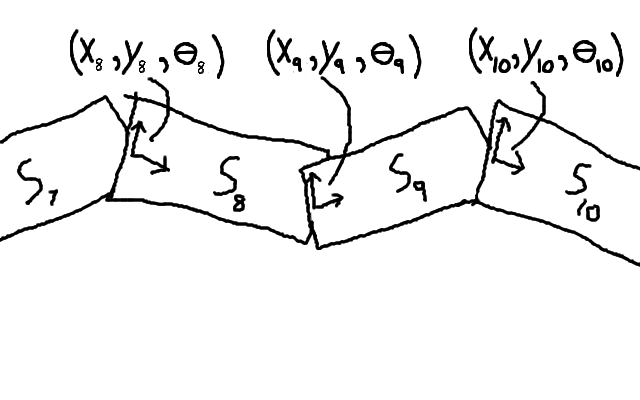
\includegraphics[scale=0.5]{3_frames_2.png}
\end{center}
\caption{Local coordinate frames attached to segments and described by reference poses.}
\label{frames2}
\end{figure}


\begin{algorithm}
\caption{Reference Pose Creation and Deactivation}          % give the algorithm a caption
\label{alg:reference}
\begin{algorithmic}

\State $N \Leftarrow 40$
\State $activeMask \Leftarrow $ array of size $N$ initialized to $0$
\State $activeRefPoses \Leftarrow $ array of size $N$ initialized to $\varnothing$
\State $preStabMask \Leftarrow \mathrm{behaviorControlOutput}()$
\State $locStabMask \Leftarrow \mathrm{stabilityCompute()}$
\For{$i = 0 \to N$} 
\If  {$preStabMask[i] \And locStabMask[i]$}
\If    {$!activeMask[i]$}
\State      $activeRefPoses[i] \Leftarrow \mathrm{computeRefPose}(i)$
\State      $activeMask[i] \Leftarrow 1$
\EndIf
\ElsIf {$activeMask[i]$}
\State    $activeRefPoses[i] \Leftarrow \varnothing$
\State    $activeMask[i] \Leftarrow 0$
\EndIf
\EndFor

\end{algorithmic}
\end{algorithm}

\begin{algorithm}
\caption{\emph{computeRefPose(i)}: Kinematics for Computing Reference Pose}
\label{alg:kinematic}
\begin{algorithmic}

\State $N \Leftarrow 40$
\State $\bar{\phi} \Leftarrow $ array of current joint angles 
\State $i \Leftarrow $ target new reference pose index
\State $j \Leftarrow $ index of nearest active reference pose to $i$

\State $k = j$
\State $(x_k, y_k, \theta_k) \Leftarrow (x_j, y_j, \theta_j)$  \Comment{pose of active reference $j$}

\If {$i > j$}
\While {$k < i$}

\State $x_{k+1} = x_k + l \cos(\theta_k)$
\State $y_{k+1} = y_k + l \sin(\theta_k)$
\State $\theta_{k+1} = \theta_k - \phi_{k+1}$
\State $k = k + 1$
\EndWhile

\ElsIf {$i < j$}
\While {$k > i$}

\State $\theta_{k-1} = \theta_k + \phi_{k-1}$
\State $x_{k-1} = x_k - l \cos(\theta_{k-1})$
\State $y_{k-1} = y_k - l \sin(\theta_{k-1})$
\State $k = k - 1$

\EndWhile
\EndIf

\State $(x_i, y_i, \theta_i) \Leftarrow (x_k, y_k, \theta_k)$ \Comment{new pose for active reference $i$}

\end{algorithmic}
\end{algorithm}

This algorithm assumes that an active reference pose always exists.  There are two special cases when no reference poses are currently active.   In the first case, the algorithm is initializing and no reference poses have been created yet.  In the second case, all of the reference poses violate the stability condition and all have been deactivated.  These special cases are not shown in the algorithms, but we explain are approach here.

For the first case, when we initialize, the first reference pose is set to $(0,0,0)$.  This becomes the origin of the global frame centered at the robot's starting position in the environment.  From this first initial reference pose, all new reference poses are derived. 

In the second case, no active reference poses are available since no stability conditions have been satisfied.  The robot has effectively lost track of its position in the environment.  In the event that a new reference pose needs to be created, there is no parent pose from which to kinematically compute.  Instead, from the last used inactive reference poses, we select the reference that was contiguously active the longest and use this as the parent pose to compute the new active reference pose.  The reasoning behind this is that a long-lived reference pose is more likely to be correct than a short-lived reference pose due to the sometimes intermittent nature of reference poses.  This last best reference pose approach is very effective in practice.  

So long as the active reference poses satisfy the assumption of no-slip anchors and there always being at least one active reference, the tracking of the robot's trajectory through the environment is correct.  Violations of these assumptions introduce error into the motion estimation.

\section{Robot-Centered Coordinate Frame}

%-N possible local coordinate systems in snake
%-none are very good to represent pose of snake because of the high variance in orientation.  Try to relate two poses to each other, orientation has almost no correlation
%-orientation is also primary source of error
%-prefer a coordinate system that represents the gross posture and pose of snake.  COM can sometimes be out of body
%-GPAC pose proposed.

\label{sec:GPAC}

Though we now have a local coordinate frame for each segment in the snake, we need a coordinate frame that represents the mobile robot body as a whole.  In traditional mobile robots, we usually have a large rigid body chassis with high inertia that is suitable for defining the position and orientation of the robot.  In a snake robot, there are multiple rigid bodies, all of which are small in mass, small in inertia, and poor at defining the overall snake's position and orientation.  While the snake is executing its locomotion, the body segments are undulating and rapidly changing orientation, making dubious their use as an indication of heading.

In the wake of these phenomena, we found the need to create a dynamically generated coordinate frame that best represents the position and orientation of the snake robot's posture as a whole.  We cannot use the center of mass of the robot, because the centroid can be outside of the body if the snake's posture is curved.  Instead, we generate a curve called a Gross Posture Approximation Curve (GPAC) that we use to generate a local coordinate frame that is oriented in the direction of travel.  This allows us to describe consecutive poses of the snake with local coordinate frames oriented in the same forward direction.

We describe in detail the GPAC and follow with the generation of the local coordinate frame.

\subsection{Gross Posture Approximation Curve (GPAC) }

The GPAC is a curve that approximates the posture of the robot in the environment without the articulation, as seen in Figure \ref{GPAC}.  The blue lines indicate the posture of the snake and the green line is the GPAC.

The GPAC is derived by taking the ordered points of the snake segment positions and fitting a smoothed B-spline curve to them.  To generate the points, we first start from a body frame fixed to one of our body segments.  In this case, we use segment 19 centered on joint 19 as our body frame $O_{19}$.  With respect to frame $O_{19}$ and using the current joint posture vector $\hat{\phi_t}$, we compute the segment posture vector $\hat{\rho_t}$ that specifies the $N$ segment poses using the iterative kinematic equations \ref{kinem1} and \ref{kinem2}.  If we take only the cartesian components of the segment posture $\bar{\rho_t}$, we set this as a series of ordered points from which we compute a B-spline curve.


\begin{figure}
  \begin{center}
    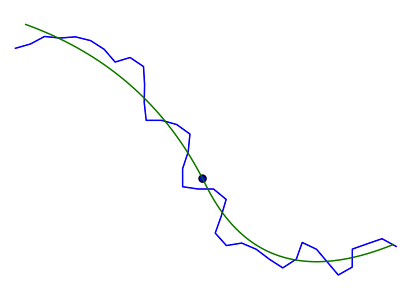
\includegraphics[scale=0.7]{plotGPAC0059.png}
  \end{center}
  \caption{Robot Posture, Gross Posture Approximation Curve (GPAC), and Local Frame Origin}
	\label{GPAC}
\end{figure}

We use the Python SciPy library's \textbf{splprep} function with a smoothness factor of $0.5$ to generate the B-spline curve.  This results in the curve shown in Figure \ref{GPAC}.  To use this curve, we define a set of parameterized functions that we use to access the curve.  First we show the function provided by the SciPy library:
\begin{equation}
O(1): \quad \beta_t(u) = ( x_u, y_u, \theta_u ),  \quad 0 \leq u \leq 1
\end{equation}

This function gives us access to the curve with a normalized parameter $u$.  The function returns the x and y coordinates of a point and the orientation of its tangent vector that correspond to the $u$ value.  The drawback to this function is that the difference of arclength between two $\beta(u)$ values is not proportional to the difference in $u$ value.  This implies that the following condition exists:
\begin{equation}
\mathbf{dist}(u_1, u_1 + K) \neq \mathbf{dist}(u_2, u_2 + K)  
\end{equation}
where the function $\mathbf{dist}()$ computes the arclength between two $u$ values on the curve, and the constant $K$ adds the same $u$ offset at two different points on the curve specified by $u_1$ and $u_2$.  What this means in practical terms is, the $u$ values cannot be relied upon to give us reproducible positions on the curve.  In particularly, if we retrieve the point $\beta_t(0.5)$, this will be close to the midpoint of the curve, but not the true midpoint and is subject to change between different curves.

We create a more accurate method that allows us to specify a point of true arclength on the curve.  We present it in the form of a parameterized function:
\begin{equation}
\label{equ:arcdist}
O(\log n): \quad \sigma_t(d) = ( x_d, y_d, \theta_d ),  \quad 0 \leq d \leq d_{max}
\end{equation}

Here $d$ is the arclength starting from the $u = 0$ terminator of the curve.  $d_{max}$ is the maximum arclength of the curve.

Though this is defined in the form of a function, it is implemented with a search algorithm.  If we pre-process the curve by uniformly pre-sampling $n$ points with $\beta_t(u)$ in $O(n)$ time, we can achieve a binary search time of $O(\log n)$ for each invocation of the function.   The $n$ parameter here corresponds to the number of samples of the curve we use to search over.  The more samples, the more accurate the function will be.   Here we use a tractable size of $n = 100$.

To perform the inverse operation for curve functions, we use the same pre-processed $n$ sample points from equation \ref{equ:arcdist} and define the following functions:
\begin{equation}
O(n): \quad \beta^{-1}_t(x, y) = u
\end{equation}
\begin{equation}
O(n): \quad \sigma^{-1}_t(x, y) = d
\end{equation}

These inverse operators find the closest sample point on the curve to $(x,y)$ and returns the sample's associated $u$ or $d$ parameter.  The correctness of these functions depend on the queried point being reasonably close to the curve, the curve not be self-intersecting, and the point not be equidistant to two disparate points on the curve.  They are $O(n)$ because we must compute the distance to all $n$ sample points.  Notice that we omit the angle portion of the curve for inverse operations.  We do not define closest point for orientations.

Since these inverse curve functions are very similar, we develop a unified algorithm that produces parallel results.  We do this to prevent duplication of search operations when similar information is needed.
\begin{equation}
O(n): \quad c_p(x,y) = (u, d, (x_p, y_p, \theta_p) )
\end{equation}

This function returns the closest point on the curve to $(x,y)$, and its associated $u$ and $d$ parameters.

Finally, we have functions that convert between $u$ and $d$.
\begin{equation}
O(\log n): \quad \mathbf{d}(u) = d
\end{equation}
\begin{equation}
O(\log n): \quad \mathbf{u}(d) = u
\end{equation}

These can be performed with a binary search on the pre-processed sample points.


\subsection{Generation of GPAC Local Frame}

%This produces a curve that approximates the general posture of the robot.  The middle point is selected by finding the location that is equidistant to the tips.  The tangent vector is used to orient the local coordinate frame.  This vector has the benefit of always pointing in the direction the robot is facing.

%and choose a point on the curve to act as our local coordinate system's origin.  This is seen in Figure \ref{GPAC}.  Notice that the direction of the curve at the origin is in the forward-backward direction making this useful as a heading reference.

For each generation of the GPAC, we can create a unique but predictable coordinate frame that represents the gross posture of the snake in the environment.  Because the GPAC only follows the general posture of the snake, regardless of its articulation, the difference in curves between generations is small and within reason.

Once we have the new GPAC, to determine the location of our new coordinate frame origin $\hat{O_t}$ with respect to $O_{19}$, we compute the following:
\begin{equation}
P_d = \sigma_t(d_{max} / 2)
\end{equation}

This specifies the halfway point along the curve in terms of arclength with respect to $O_t$.  If we had used $\beta_t(0.5)$ instead, we would have had no guarantee how close to the middle it would be and no guarantees on repeatibility.  By using the arclength function $\sigma_k()$, we have more guarantee over the location at the expense of running time.

From our new local frame $\hat{O_t}$, the orientation of the x-axis is directed in the forward direction of the snake, regardless of the articulation of the joints.  This approach now gives us the tools to make relations between snake poses where the orientations will have some correlation.  If we had insisted on using a body frame $O_{19}$ as a local coordinate frame, the orientations would have had very little correlation.  We would have had no means to relate and correct orientations between snake poses.

In the future, we will drop the $t$ subscript of a GPAC and local frame origin and only refer to them as $\beta_k(u)$, $\hat{O}_k$, and $\hat{P}_k$, where $\hat{O}_k$ is the  GPAC generated origin, $\hat{P}_k$ is the origin's location in the global frame, and $k$ is the particular pose number in the pose graph.  We describe this in more detail in Section 5.

\subsection{Geometric Transform between Poses}

\label{sec:geo_transform}

Now that we have defined a local coordinate system for the complete posture of a snake robot, we can compute a geometric transform $T_{ij}$ between two poses of the robot $\hat{P}_i$ and $\hat{P}_j$.  We take the snake poses before and after one step of the adaptive concertina gait in the GPAC local frame for each.  Each GPAC has a reference pose in the global frame, so it is only a matter of computing a transform between the two.

\section{Results}

Shown in Figure \ref{varWidth} is a plot of the snake robot¿s poses as it travels through a variable width curved pipe.  The boundaries of the pipe are drawn in green.  The black poses represent the estimated positions and the pink poses indicate the ground truth positions.  Notice that there is a discontinuity in the middle, which is likely because of the use of a reference node on an anchor with major slip.  Also, notice the sudden rotation and translation at the end caused by the slip from hitting the termination wall.   Here we do not show our collision detection and correction system, so the error introduced from the collision is shown in the plot.

Figure \ref{juncFix} showns the trajectory plot of the snake robot through a fixed-width environment with junctions.  This shows that the motion estimation has no problems estimating motion through junctions so long as the anchors are good.
 
\begin{figure}
  \begin{center}
    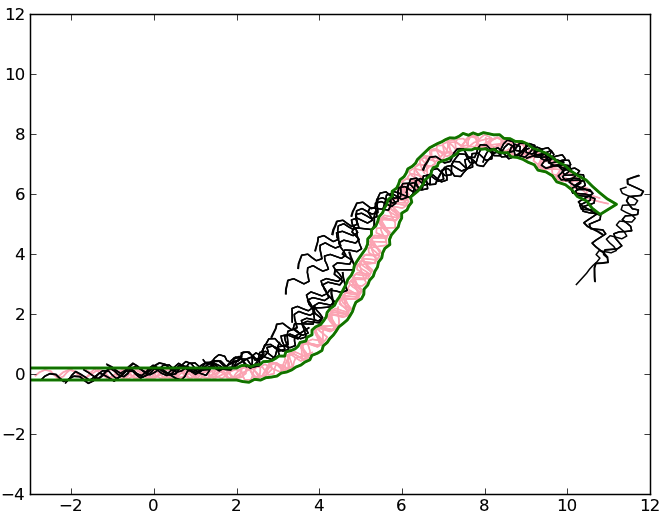
\includegraphics[width=3.4in]{plotMotionVariableWidth.png}
  \end{center}
  \caption{Estimated Trajectory of Robot through Variable-Width Pipe}
	\label{varWidth}
\end{figure}

\begin{figure}
  \begin{center}
    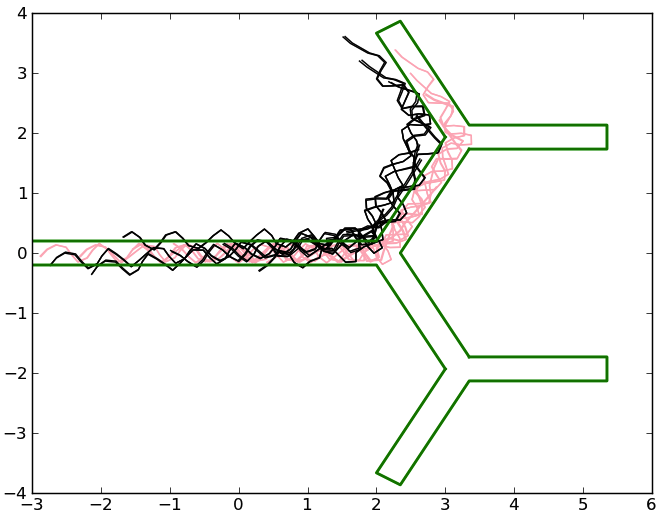
\includegraphics[width=3.4in]{plotMotionJunctions.png}
  \end{center}
  \caption{Estimated Trajectory of Robot through Fixed-Width Pipe with Junctions}
	\label{juncFix}
\end{figure}

In spite of the care taken in locomotion and motion estimation, the snake robot still accumulates positional errors.  The primary cause of this is the failure of anchors.   This can happen by the anchor originally failing to take hold, intermittent anchor motion or slip, or anchor slip caused by collision with a forward obstacle making a backward motion look like a forward motion.



The quality of motion estimation is a function of how slowly and carefully we perform our movements and maintain our anchors.  Particularly, the parameters we tune for our local stability detection and the rate of linear interpolation for movement transitions.



